\documentclass[pdflatex,referee,sn-basic]{sn-jnl}% Basic Springer Nature reference style; referee = double spacing
% Line numbers on the text lines (lineno package). The class's own `lineno' option draws a fixed margin ruler
% at single-spacing pitch, which with double spacing gives two numbers per line and numbers beside blank space.
\usepackage[left,mathlines]{lineno}

\usepackage{graphicx}%
\usepackage{multirow}%
\usepackage{amsmath,amssymb,amsfonts}%
\usepackage{amsthm}%
\usepackage[title]{appendix}%
\usepackage{xcolor}%
\usepackage{booktabs}%
\usepackage{array}%
\usepackage{tikz}
\usepackage{pgfplots}
\usepackage{scalerel}
\usetikzlibrary{positioning, decorations.pathreplacing, calligraphy, calc, shapes.geometric, intersections, arrows}
\usepgfplotslibrary{fillbetween}
\pgfplotsset{compat=1.18}

\newcommand{\fmri}{functional magnetic resonance imaging}
\newcommand{\FMRI}{Functional magnetic resonance imaging}
\newcommand{\fmriabbrv}{fMRI}
\newcommand{\eeg}{electroencephalography}
\newcommand{\EEG}{Electroencephalography}
\newcommand{\eegabbrv}{EEG}

% float placement: fewer half-empty pages around large floats
\renewcommand{\topfraction}{0.9}\renewcommand{\bottomfraction}{0.8}\renewcommand{\textfraction}{0.07}
\renewcommand{\floatpagefraction}{0.85}\renewcommand{\dbltopfraction}{0.9}\renewcommand{\dblfloatpagefraction}{0.85}
\setcounter{topnumber}{3}\setcounter{bottomnumber}{2}\setcounter{totalnumber}{5}
\raggedbottom

\begin{document}
\linenumbers

\title[Benchmarking EEG-to-fMRI synthesis for diagnosis]{What Does EEG-to-fMRI Synthesis Add to EEG-Based Diagnosis? A Controlled Benchmark in Psychosis, Schizophrenia and Parkinson's Disease}

\author*[1]{\fnm{David} \sur{Calhas}}\email{davidcalhas@gmail.com}
\author[2]{\fnm{Rui} \sur{Henriques}}\email{rmch@tecnico.ulisboa.pt}

\affil*[1]{\orgdiv{Faculty of Computer and Information Science}, \orgname{University of Ljubljana}, \orgaddress{\city{Ljubljana}, \country{Slovenia}}}
\affil[2]{\orgdiv{INESC-ID, Instituto Superior T\'{e}cnico}, \orgname{Universidade de Lisboa}, \orgaddress{\city{Lisbon}, \country{Portugal}}}

\abstract{\textbf{Background:} Synthesis of functional magnetic resonance imaging (fMRI) from electroencephalography (EEG) has been proposed to support EEG-only diagnosis, but whether synthesized fMRI adds information beyond the EEG it is computed from has not been tested with appropriate controls.

\textbf{Methods:} Four synthesizers were trained on two simultaneous EEG-fMRI datasets of healthy adults and applied to resting EEG from five public cohorts: two first-episode psychosis samples (77 and 61 participants), chronic schizophrenia (77), Parkinson's disease (50) and a task-EEG schizophrenia-spectrum sample (43). Synthesized fMRI was compared with EEG band power and with an EEG view matched in information to the synthesizer input, alone and combined, under nested repeated cross-validation, permutation tests and Holm-corrected paired bootstrap; untrained (random-weight) synthesizers controlled for architecture.

\textbf{Results:} Band power separated Parkinson's disease from controls (area under the ROC curve, AUC, 0.79) but not the psychosis or schizophrenia cohorts (0.54--0.65); the information-matched view reached 0.83. Synthesized views classified Parkinson's disease (best AUC 0.74), but untrained synthesizers matched them (0.69--0.74) and no trained synthesizer added to the information-matched view in any cohort. The only gain surviving correction came from an untrained network in chronic schizophrenia and disappeared after ocular-artefact removal. The synthesizers did not outperform an EEG-free template image, and EEG explained a negligible part of the blood-oxygen-level-dependent signal (correlation 0.03).

\textbf{Conclusions:} Current synthesized fMRI is a transform of EEG spectra whose learned mapping added no diagnostic information. The protocol, code and checklist of controls set a baseline for future diagnostic claims.}

\keywords{Electroencephalography, EEG-to-fMRI synthesis, Functional MRI, Schizophrenia, First-episode psychosis, Parkinson's disease, Diagnostic classification, Cross-modal generation, Benchmark, Evaluation protocol}

\maketitle

\section{Introduction}\label{section:introduction}

Functional MRI resolves brain activity in space but is costly and scarce \cite{ogbole2018survey}; EEG is cheap and portable but spatially coarse. EEG-to-fMRI synthesis learns, from simultaneous recordings, a mapping from scalp EEG to BOLD volumes or region time series \cite{liu2019convolutional, liu2020latent, bricman2021eeg2fmri, calhas2022eeg, roos2025brainwaves, he2025spec2vol, lanzino2024ntvit, yao2025catd, li2024neurobolt, li2026unebolt}, and has been proposed as a way to obtain fMRI-like information where only EEG is available. Psychotic disorders and Parkinson's disease are natural targets: both show EEG and fMRI group differences \cite{tan2016eeg, roach2008event, bates2009low, oh2020identifying, velakoulis2006hippocampal, haukvik2013schizophrenia}, and patients have been classified from synthesized fMRI in schizophrenia, in an earlier version of this work \cite{calhas2023medrxiv}, and in Parkinson's disease \cite{yao2025catd}.

A synthesizer cannot create information absent from its EEG input. Its potential value for diagnosis lies in representation: a mapping learned from simultaneous recordings could act as a prior that makes group differences linearly accessible to a classifier trained on the 50--80 subjects of a typical clinical cohort. Testing this requires controls that, to our knowledge, have not been applied together: data without acquisition differences between groups; EEG-only views under identical validation, including one that receives the same spectral information as the synthesizer; combinations of EEG and synthesized views; and untrained networks, which separate the learned mapping from the inductive bias of the architecture.

\textbf{Contributions.} (1) An evaluation protocol for diagnostic claims from synthesized fMRI: harmonisation of any clinical EEG onto the synthesizers' training montage; EEG-only baselines, one of them matched in information to the synthesizer input; fusion tests; untrained-network controls; artefact and recording-condition checks; and subject-level permutation and corrected bootstrap inference. (2) A benchmark applying it to four synthesizers (the convolutional neural network with topographical attention graph, CNN-TAG \cite{calhas2022eeg}, E2fNet, Spec2VolCAMU-Net and NT-ViT), trained on two simultaneous EEG-fMRI datasets, and to a contrastive fine-tuning method \cite{calhas2023medrxiv}, on five public cohorts of first-episode psychosis, chronic schizophrenia, a schizophrenia-spectrum task cohort and Parkinson's disease. (3) Evidence on what the synthesizers learn, against an EEG-free template and a fair BOLD target. (4) A checklist of controls (Table~\ref{tab:checklist}) and open code.

\section{Materials and methods}\label{section:methods}

\subsection{Datasets and design}\label{materials:data}

Figure~\ref{fig:overview} summarises the design and Table~\ref{tab:data_description} the datasets, all previously published anonymised public releases analysed as secondary data. Synthesizers were trained on NODDI \cite{dataset_01,deligianni2016}, 16 healthy adults recorded at rest with simultaneous EEG-fMRI (1.5\,T, TR 2.16\,s), and, to test dependence on the training data, on XP1 \cite{lioi2020xp}, ten healthy adults (3\,T, TR 2\,s, motor imagery and neurofeedback). The clinical cohorts are two independent first-episode psychosis samples (FEP1, FEP2; OpenNeuro ds003944 and ds003947) \cite{salisbury_ds003944,salisbury_ds003947}, in which five people recorded twice in FEP1 were kept once; chronic schizophrenia (Semmelweis) \cite{racz2025}, with patients identified by their PANSS ratings; Parkinson's disease (ds003490, OFF-medication session) \cite{cavanagh_ds003490}; and a schizophrenia-spectrum cohort recorded during an Ultimatum Game (Fribourg, ds004000) \cite{dataset2022fribourg,horat2018impaired}, the cohort of \cite{calhas2023medrxiv}. Cohort details and data checks are in Additional file~1 (Section~S1).

\begin{figure*}[!tbp]
    \centering
    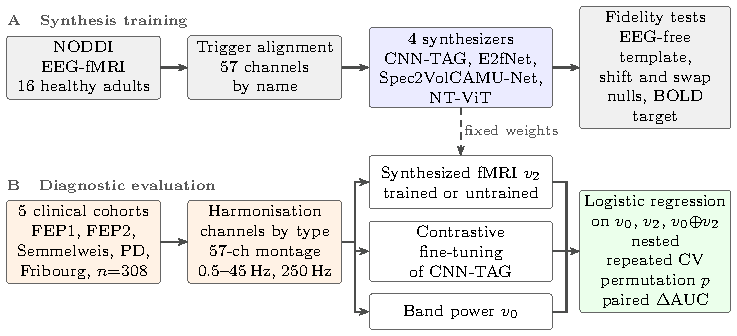
\includegraphics[width=\textwidth]{fig1.pdf}
    \caption{\textbf{Study design.} Four synthesizers are trained on simultaneous EEG-fMRI of healthy adults (NODDI) with scanner-trigger alignment and kept fixed. Resting EEG of five clinical cohorts is harmonised to the training montage and represented by band power ($v_0$), by the synthesized fMRI of each synthesizer with learned or random weights ($v_2$), and by their combination ($v_0\oplus v_2$); a contrastive fine-tuning of CNN-TAG is evaluated alongside. Every view is classified with the same nested cross-validation and permutation tests. Supporting analyses on NODDI test what the synthesizers learn.}
    \label{fig:overview}
\end{figure*}

\begin{table}[!tbp]
    \centering
    \caption{Characteristics and roles of the datasets. \textit{pt}: patients; \textit{hc}: healthy controls; age as mean $\pm$ standard deviation (years); analysed EEG is the fixed crop used for every subject of a cohort.}
    \label{tab:data_description}
    \small
    \begin{tabular}{p{1.75cm} | p{1.95cm} | p{0.85cm} | p{2.0cm} | p{1.3cm} | p{2.65cm}}
        \hline
        \hline
         \hfil Dataset & \hfil Role / disease & \hfil pt/hc & \hfil Age pt | hc & \hfil Sex (M/F) pt | hc & \hfil Recording (analysed EEG) \\
         \hline
         NODDI & synthesis training & 0/16 & \hfil $32.8\pm8.1^{a}$ & \hfil 11/6$^{a}$ & rest, eyes open, simultaneous EEG-fMRI, 64 ch, 250\,Hz \\
         FEP1 (ds003944) & first-episode psychosis & 47/30 & $22.5\pm5.1$ | $21.6\pm4.1$ & 33/14 | 18/12 & rest, eyes open, 61 ch, 1\,kHz (300\,s) \\
         FEP2 (ds003947) & first-episode psychosis & 31/30 & $23.4\pm4.7$ | $24.2\pm5.1$ & 22/9 | 16/14 & rest, eyes open, 61 ch, 1\,kHz (300\,s) \\
         Semmelweis & schizophrenia (chronic) & 38/39 & $33.9\pm10.6$ | $32.7\pm9.7$ & 24/14 | 24/15 & rest, eyes closed, 64 ch, 1\,kHz (118\,s$^{b}$) \\
         PD (ds003490) & Parkinson's disease (OFF) & 25/25 & $69.7\pm8.7$ | $69.3\pm9.6$ & 16/9 | 16/9 & rest, eyes closed/open spans, 63 ch, 500\,Hz (400\,s) \\
         Fribourg (ds004000) & schizophrenia spectrum & 19/24 & n/a & n/a & Ultimatum Game, 128 ch, 2048\,Hz (400\,s) \\
         \hline
         \hline
    \end{tabular}

    \raggedright\footnotesize $^{a}$For the 17 acquired participants; version 2 of the release contains 16. $^{b}$One control recording is 109.7\,s long and was used in full.
\end{table}

\subsection{Pairing EEG and fMRI}\label{section:fmri_data}

In NODDI the EEG export begins 13--130\,s before the first volume in 15 of 16 subjects and two electrode montages are present, so EEG and volumes were paired through the scanner markers and the 57 channels recorded in all subjects were selected by name. In XP1 the number of raw scanner triggers differed from the number of volumes in 15 of 35 runs; only the 19 runs with one trigger per volume were used (all ten subjects; 2,552 training and 669 validation volumes), and volumes were resampled to the $64\times64\times30$ grid of NODDI (Additional file~1, Section~S2).

\subsection{EEG harmonisation and artefact handling}\label{section:adaptation}

Every recording went through one harmonisation (MNE-Python): EEG channels selected by declared type (EOG, ECG, EMG, accelerometer and auxiliary channels removed, which also removes the group-dependent auxiliary layout of the Fribourg release), spherical-spline interpolation onto the 57 NODDI channels, mains notch, 0.5--45\,Hz band-pass, average reference, 250\,Hz, and a fixed crop per cohort, identical for patients and controls. Synthesizers were applied to consecutive pseudo-TRs of 2.16\,s starting 43.2\,s into each recording. The primary analysis used no artefact rejection. As sensitivity analyses, every recording was re-harmonised with independent component analysis (ICA), removing EOG-correlated components (using EOG channels present in every recording of a cohort, so that cleaning cannot differ by group through the channel set); band power was recomputed without the muscle-sensitive 30--45\,Hz band; and in Parkinson's disease, whose rest file contains a set-up period, one minute each of eyes closed and eyes open and then an auditory oddball task, a crop restricted to the rest spans was analysed. Artefact measures and recording metadata were compared between groups (Additional file~1, Section~S3).

\subsection{EEG views and synthesizers}\label{eeg_views:eeg_to_fmri}

The band-power view $v_0$ is the Welch relative log power of each channel in five bands (1--4, 4--8, 8--13, 13--30 and 30--45\,Hz) \cite{roach2008event,bates2009low}. The synthesizers receive log-magnitude spectra of 20 consecutive 2.16\,s segments (57 channels $\times$ 97 bins), the 43.2\,s of EEG that precede a volume and cover the haemodynamic delay. Two EEG views are matched in information to this input: the temporal mean and standard deviation over a recording's pseudo-TRs of the input spectra ($v_1^{\mathrm{ms}}$), and the same summary of an untrained sparse random projection \cite{li2006sparse} of each pseudo-TR's complete input. The synthesized-fMRI view $v_2$ is the voxelwise temporal mean and standard deviation of a subject's synthesized volumes.

The four synthesizers are CNN-TAG \cite{calhas2022eeg}, from our earlier work (Additional file~1, Fig.~S1), E2fNet \cite{roos2025brainwaves}, Spec2VolCAMU-Net \cite{he2025spec2vol} and NT-ViT \cite{lanzino2024ntvit}; CATD \cite{yao2025catd} has no public code, and NeuroBOLT and UnEBOLT \cite{li2024neurobolt,li2026unebolt} predict region time series and were used for fidelity only. They were trained on min--max-scaled EPI volumes with $0.5(1-\mathrm{SSIM})+0.5\,\mathrm{MSE}$ (NT-ViT with its authors' recipe), with the epoch selected on two held-out subjects: 11 for E2fNet, 10 for Spec2VolCAMU-Net, 20 for NT-ViT and the first epoch for CNN-TAG, whose validation SSIM did not improve afterwards; a CNN-TAG trained for 50 epochs was therefore evaluated as well. Untrained controls apply the same architectures with random weights through the identical pipeline. We also evaluated the integration method of the earlier version of this work \cite{calhas2023medrxiv}, which fine-tunes the CNN-TAG encoder with a contrastive loss on its layer-normalised Fourier-feature space while a linear classifier is trained on the synthesized volume and the decoder stays fixed (Additional file~1, Section~S5).

\subsection{Classification and statistics}\label{section:setting}

Each view was classified with an $l_2$-regularised logistic regression \cite{treviso2020explanation} under repeated stratified 10-fold cross-validation at the subject level (20 repeats; 3 for the contrastive classifier), with the regularisation strength chosen by inner 5-fold cross-validation; standardisation and principal components (20 for high-dimensional blocks, computed exactly from the subject Gram matrix) were fitted on training folds only. We report the mean AUC over repeats with a 95\% bootstrap interval over subjects and a one-sided label-permutation $p$-value (1,000 permutations for EEG views, 500 for synthesized views and 20, exploratory, for the contrastive classifier; each permutation re-runs the nested procedure with two repeats, which is conservative). The added value of synthesis is the $\Delta$AUC of the combined view ($v_0\oplus v_2$ or $v_1^{\mathrm{ms}}\oplus v_2$) over the EEG view, estimated with a paired stratified bootstrap (20,000 resamples) and Holm-adjusted within the 20 trained-synthesizer and the 40 trained-or-untrained comparisons of each baseline. Sensitivity analyses varied the number of components (5, 10, 40) and pooling, regressed covariates out of every feature within training folds (age and sex; medication dose in the psychosis cohorts; recording hour in Semmelweis and Fribourg; recording year in Fribourg), and used ICA-cleaned inputs, the Parkinson's disease rest crop, XP1-trained synthesizers and the 50-epoch CNN-TAG. Leave-one-subject-out estimation was not used, because it biases weak features below chance \cite{varoquaux2018}.

\subsection{What the synthesizers learn}\label{setting:fidelity}

On NODDI, leave-one-subject-out fidelity (SSIM, PSNR and voxelwise temporal correlation, against circularly shifted EEG) was compared with that of an EEG-free template (the mean training volume), with trigger-aligned EEG, EEG paired from the file start and ECG alone. A fair target, motion-corrected BOLD cleaned with Friston-24 and spike regressors \cite{friston1996,power2014} and averaged in 48 cortical parcels, tested how much BOLD variance EEG predicts (ridge regression and UnEBOLT \cite{li2026unebolt,jiang2024labram}) against shift, swap and IAAFT surrogate nulls \cite{schreiber1996,mehta2025time} (Additional file~1, Section~S7).

\subsection{Ethics approval and use of language models}\label{section:ethics}

This is a secondary analysis of anonymised public data; all original studies were approved by the responsible committees and obtained informed consent: NODDI, approval ID 4290/001 \cite{dataset_01}; first-episode psychosis, University of Pittsburgh Institutional Review Board \cite{salisbury_ds003944,salisbury_ds003947}; Semmelweis, Semmelweis University Regional and Institutional Committee of Science and Research Ethics, registration number 197/2015 \cite{racz2025}; Parkinson's disease, University of New Mexico Office of the Institutional Review Board \cite{cavanagh_ds003490}; Fribourg, approval ID 054/13-CER-FR \cite{dataset2022fribourg}; XP1 \cite{lioi2020xp}. A large language model (Claude, Anthropic) was used to assist with writing analysis code and drafting and editing the manuscript text; all analyses, results and text were reviewed and verified by the authors, who take full responsibility for the content.

\section{Results}\label{section:results}

\subsection{Classification}\label{section:res_clf}

Band power separated Parkinson's disease from controls (AUC $0.786$, 95\% CI $0.63$--$0.92$, $p=0.002$) but not the psychosis or schizophrenia cohorts (Table~\ref{tab:auc}, Fig.~\ref{fig:results}; FEP1 $0.620$, $p=0.07$; FEP2 $0.646$, $p=0.050$; Semmelweis $0.571$; Fribourg $0.539$; FEP1 and FEP2 pooled $0.568$, consistent with heterogeneity between the samples). The information-matched view was the best single view in Parkinson's disease ($0.825$, $p=0.001$; random projection $0.823$) and did not exceed band power elsewhere. Trained synthesizers discriminated in Parkinson's disease (E2fNet $0.744$, Spec2VolCAMU-Net $0.694$, NT-ViT $0.672$; CNN-TAG $0.483$) without reaching band power, and their untrained versions did as well ($0.69$--$0.74$). In the psychosis and schizophrenia cohorts no trained synthesizer was significant. CNN-TAG in FEP2 fell to $0.329$: its components were unrelated to any recording or clinical variable, and its inner cross-validation AUC was below $0.5$ in every fold while the training AUC was $0.71$--$0.83$, the signature of anti-learning in features without signal (Additional file~1, Section~S6).

\begin{table}[!tbp]
    \centering
    \caption{AUC of every view (mean over 20 repeats of stratified 10-fold cross-validation). Synthesized views: trained / untrained (random-weight) synthesizer. $^{*}$One-sided permutation $p<0.05$ (1,000 permutations for EEG views, 500 for synthesized views). Intervals and $p$-values are in Additional file~2.}
    \label{tab:auc}
    \scriptsize\setlength{\tabcolsep}{2.5pt}
    \begin{tabular}{@{}l c c c c c c@{}}
        \hline
        & Band & Information- & CNN-TAG & E2fNet & Spec2Vol- & NT-ViT \\
        Cohort & power & matched EEG & & & CAMU-Net & \\
        \hline
        FEP1 & $0.62$ & $0.52$ & $0.57$ / $0.41$ & $0.53$ / $0.63$ & $0.60$ / $0.52$ & $0.50$ / $0.60$ \\
        FEP2 & $0.65^{*}$ & $0.57$ & $0.33$ / $0.55$ & $0.57$ / $0.57$ & $0.61$ / $0.57$ & $0.60$ / $0.63^{*}$ \\
        Semmelweis & $0.57$ & $0.54$ & $0.58$ / $0.56$ & $0.53$ / $0.47$ & $0.62$ / $0.74^{*}$ & $0.47$ / $0.57$ \\
        PD & $0.79^{*}$ & $0.83^{*}$ & $0.48$ / $0.70^{*}$ & $0.74^{*}$ / $0.71^{*}$ & $0.69^{*}$ / $0.74^{*}$ & $0.67^{*}$ / $0.69^{*}$ \\
        Fribourg & $0.54$ & $0.56$ & $0.60$ / $0.55$ & $0.54$ / $0.54$ & $0.61$ / $0.49$ & $0.63$ / $0.53$ \\
        \hline
    \end{tabular}
\end{table}

\begin{figure}[!t]
    \centering
    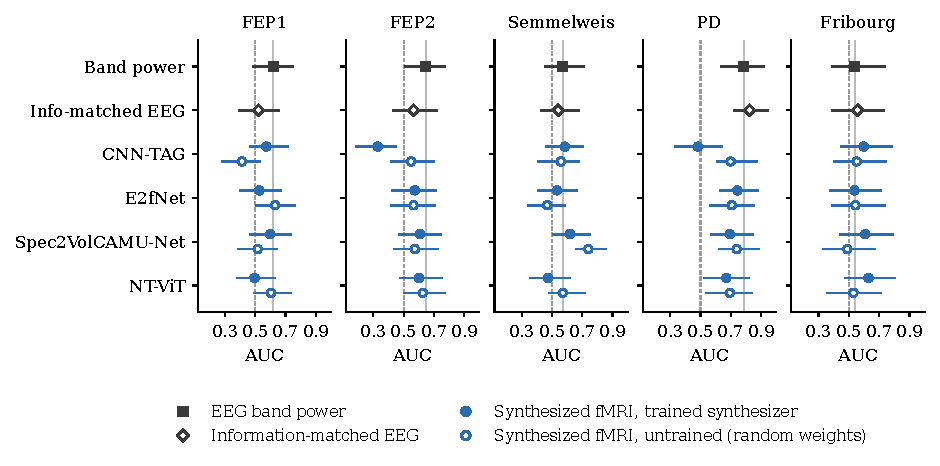
\includegraphics[width=\textwidth]{fig2.pdf}
    \caption{\textbf{Classification AUC by cohort and view.} Mean AUC over 20 repeats of stratified 10-fold cross-validation with 95\% bootstrap intervals, for EEG band power (squares), the information-matched EEG view (open diamonds) and the synthesized fMRI view of each synthesizer with learned weights (filled circles) or random weights (open circles). Dashed line: chance; grey line: band-power AUC. FEP1, FEP2: first-episode psychosis; Semmelweis: chronic schizophrenia; PD: Parkinson's disease; Fribourg: schizophrenia spectrum, task EEG.}
    \label{fig:results}
\end{figure}

\subsection{Added value of synthesized fMRI}\label{section:res_delta}

Added to band power, no trained synthesizer gave a gain that survived Holm correction. Nominal gains (Spec2VolCAMU-Net $+0.035$ and NT-ViT $+0.038$ in Parkinson's disease; E2fNet $+0.067$ and Spec2VolCAMU-Net $+0.112$ in Semmelweis; E2fNet $+0.075$ in Fribourg) were matched where the EEG carried signal by adding the information-matched view instead ($+0.030$ in Parkinson's disease). Added to the information-matched view, no trained synthesizer improved classification in any cohort; the only trained-synthesizer difference that survived correction was a loss (CNN-TAG in FEP2, $-0.226$). Among the untrained networks, Spec2VolCAMU-Net in Semmelweis added $+0.165$ (95\% CI $+0.089$ to $+0.248$) over band power and $+0.169$ ($+0.073$ to $+0.265$) over the information-matched view, the only gain that survived correction across 40 comparisons (Additional file~2, Table~S1).

\subsection{Sensitivity, artefacts and recording conditions}\label{section:res_sens}

No sensitivity analysis brought a trained synthesizer above the information-matched view (Table~\ref{tab:sens}). XP1-trained synthesizers reached AUC $0.34$--$0.68$; the 50-epoch CNN-TAG $0.65$ in Parkinson's disease and $0.74$ in Semmelweis; single synthesized views varied by up to $0.4$ AUC with the number of components. Regressing out covariates left Parkinson's disease unchanged (band power $0.80$, information-matched $0.83$) and lowered the untrained Spec2VolCAMU-Net in Semmelweis to $0.62$. Removing ocular components by ICA also left Parkinson's disease unchanged ($0.81$ and $0.80$), but lowered band power in FEP1 ($0.54$) and FEP2 ($0.58$) and abolished the Semmelweis effect ($0.57$, $p=0.13$); after ICA no gain survived correction in any cohort. In Parkinson's disease, the rest-only crop kept band power at $0.81$ ($0.82$ after ICA); there the trained CNN-TAG ($0.81$) outperformed its untrained version ($0.57$), the only such case, but still added nothing to band power ($+0.013$, 95\% CI $-0.018$ to $+0.045$).

Recording conditions differed by group in three cohorts (Additional file~2, Table~S3). In Parkinson's disease controls showed more ocular activity than patients ($p=0.004$), consistent with reduced blinking in Parkinson's disease, whereas accelerometer power did not differ; all recordings followed the same order (eyes closed, eyes open, task) with group-independent timing. Semmelweis patients were recorded earlier in the day ($p<0.001$) and had more high-amplitude segments ($p=0.003$); in Fribourg the participants recorded in 2016 were all patients. The number of ocular components removed by ICA did not differ between groups in any cohort.

The contrastive classifier discriminated only in Parkinson's disease (re-initialised encoder $0.701$, exploratory $p=0.048$), below band power, and starting from the NODDI-trained encoder gave no advantage (Additional file~2, Table~S4).

\begin{table}[!tbp]
    \centering
    \caption{Sensitivity analyses: AUC of the best synthesized view (syn., maximum over the four synthesizers, which favours synthesis) and of the information-matched EEG view (EEG) under the same analysis.}
    \label{tab:sens}
    \scriptsize\setlength{\tabcolsep}{2.5pt}
    \begin{tabular}{@{}l cc cc cc cc cc@{}}
        \hline
        & \multicolumn{2}{c}{FEP1} & \multicolumn{2}{c}{FEP2} & \multicolumn{2}{c}{Semmelweis} & \multicolumn{2}{c}{PD} & \multicolumn{2}{c}{Fribourg} \\
        Analysis & syn. & EEG & syn. & EEG & syn. & EEG & syn. & EEG & syn. & EEG \\
        \hline
        Primary (NODDI) & $0.60$ & $0.52$ & $0.61$ & $0.57$ & $0.62$ & $0.54$ & $0.74$ & $0.83$ & $0.63$ & $0.56$ \\
        Untrained & $0.63$ & $0.52$ & $0.63$ & $0.57$ & $0.74$ & $0.54$ & $0.74$ & $0.83$ & $0.55$ & $0.56$ \\
        Trained on XP1 & $0.63$ & $0.52$ & $0.57$ & $0.57$ & $0.66$ & $0.54$ & $0.68$ & $0.83$ & $0.54$ & $0.56$ \\
        CNN-TAG 50 epochs & $0.49$ & $0.52$ & $0.48$ & $0.57$ & $0.74$ & $0.54$ & $0.65$ & $0.83$ & $0.66$ & $0.56$ \\
        5--40 comp., pooling & $0.65$ & $0.52$ & $0.62$ & $0.57$ & $0.68$ & $0.54$ & $0.74$ & $0.83$ & $0.67$ & $0.56$ \\
        Covariates removed & $0.60$ & $0.52$ & $0.59$ & $0.55$ & $0.63$ & $0.53$ & $0.75$ & $0.83$ & $0.62$ & $0.49$ \\
        ICA (ocular) & $0.62$ & $0.55$ & $0.54$ & $0.54$ & $0.63$ & $0.49$ & $0.70$ & $0.80$ & $0.62$ & $0.65$ \\
        \hline
    \end{tabular}
\end{table}

\subsection{What the synthesizers learn}\label{section:res_fidelity}

On NODDI, the EEG-free template reached SSIM $0.675$ ($0.676$ in E2fNet's own pipeline), above the published values of E2fNet ($0.605$) and NT-ViT ($0.581$) and slightly below that of Spec2VolCAMU-Net ($0.693$), which come from each study's own split. Retrained with trigger-aligned EEG, ridge regression, CNN-TAG and E2fNet were below the template on SSIM ($0.631$--$0.655$, $p\leq0.003$), Spec2VolCAMU-Net tied it ($0.679$, $p=0.30$), and all were worse on RMSE ($p\leq0.0002$); EEG from the file start or ECG alone changed little, no model showed a temporal correlation above shifted EEG, and the final and XP1-trained synthesizers behaved the same on held-out subjects (Additional file~2, Table~S5). Figure~\ref{fig:examples} shows why: Spec2VolCAMU-Net and NT-ViT produce an almost constant, template-like volume, E2fNet varies mainly at the brain edge, and the one-epoch CNN-TAG fluctuates without following the real signal, so a synthesizer's output differs between subjects mainly through the subject's overall EEG spectrum. With the fair target, EEG predicted a detectable but negligible part of BOLD in held-out subjects (ridge $r=0.026$, UnEBOLT $r=0.035$, above shift and swap nulls; $R^2\approx0$).

\begin{figure*}[!tbp]
    \centering
    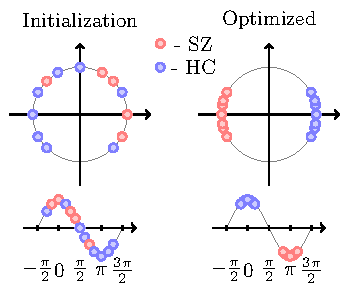
\includegraphics[width=0.88\textwidth]{fig3.pdf}
    \caption{\textbf{Synthesized volumes of a held-out subject.} NODDI subject 49 (held out from training), final synthesizers used for the clinical cohorts. \textbf{A} One volume (axial slice 15 of 30) of the real data, the EEG-free template and each synthesizer. \textbf{B} Voxelwise temporal standard deviation over the 287 volumes (same scale for all). \textbf{C} Brain-mean intensity over time, demeaned, on the same intensity scale.}
    \label{fig:examples}
\end{figure*}

\section{Discussion}\label{section:discussion}

\noindent\textbf{Synthesized fMRI did not add diagnostic information beyond its EEG.} Across four synthesizers trained on two datasets and five clinical cohorts, no trained synthesizer improved classification over an EEG view given the same spectral information, none of their gains over band power survived correction, and where synthesized views discriminated, most clearly in Parkinson's disease, random-weight networks did as well. Retraining on a second dataset, training CNN-TAG to convergence, changing the dimensionality reduction, regressing out covariates and removing ocular artefacts did not change this.

\begin{table}[!tbp]
    \centering
    \caption{Controls for diagnostic claims from synthesized fMRI: the alternative explanation each rules out, and what it showed in this study.}
    \label{tab:checklist}
    \scriptsize\setlength{\tabcolsep}{3pt}
    \begin{tabular}{@{}>{\raggedright\arraybackslash}p{6.0cm}>{\raggedright\arraybackslash}p{6.6cm}@{}}
        \hline
        Control (alternative explanation ruled out) & In this study \\
        \hline
        EEG-only baseline under identical validation (synthesis adds nothing beyond its EEG) & Band power above every synthesized view in Parkinson's disease \\
        EEG view matched in information to the synthesizer input (gain from a richer EEG summary) & Best single view in Parkinson's disease; no trained synthesizer added to it \\
        Fusion test with correction for multiplicity (chance gains among many comparisons) & No trained-synthesizer gain survived Holm correction \\
        Untrained-network control (inductive bias of the architecture) & Untrained matched trained synthesizers in Parkinson's disease; the one surviving gain came from an untrained network \\
        Channel selection by type; metadata checks (recording set-up differs by group) & Auxiliary channels and recording year (Fribourg), time of day (Semmelweis) \\
        ICA and artefact measures by group (ocular, muscle or movement artefacts) & Ocular activity differed in Parkinson's disease; the surviving gain vanished after ICA \\
        A crop with the same content in every recording (task or set-up periods) & The Parkinson's disease rest file contained a set-up period and an oddball task \\
        Subject-level nested cross-validation and permutation tests (leakage, tuning on test data, anti-learning) & All estimates subject-level, with permutation $p$ \\
        EEG-free template; shift and swap nulls (fidelity that reflects anatomy, not EEG timing) & Template matched or exceeded all synthesizers; voxelwise $r\approx0$ \\
        Trigger alignment and channels by name (EEG paired with the wrong volumes or electrodes) & NODDI EEG starts 13--130\,s before the first volume; XP1 triggers $\neq$ volumes in 15 of 35 runs \\
        \hline
    \end{tabular}
\end{table}

\noindent\textbf{Representation, not information.} The controls separate three possible sources of a gain: a richer EEG summary (the information-matched view), the architecture's inductive bias (untrained networks) and the learned mapping (trained against untrained). Every gain came from the first two. The one gain that survived correction, an untrained Spec2VolCAMU-Net in chronic schizophrenia, looked like an architecture effect but shrank with recording hour, disappeared after ICA and was not reproduced by the trained networks; it most likely reflects ocular artefacts and recording conditions that differ between the groups of that cohort.

\noindent\textbf{Why the learned mapping adds nothing.} The synthesizers reproduce the static anatomy of an EEG-free template, and their outputs differ between subjects mainly through each subject's EEG spectrum: their subject-level summaries are nonlinear transforms of the spectra that the information-matched view summarises linearly. As EEG predicts a negligible share of BOLD variance even with a state-of-the-art model, a diagnostic gain from the learned mapping would not be expected.

\noindent\textbf{Scope and recording conditions.} These conclusions concern current volumetric synthesizers trained on small healthy datasets and applied to clinical EEG that differs from the training data in system, montage, eye state and, in one cohort, paradigm; they do not exclude that synthesizers trained on larger or clinical simultaneous data, with an EEG-dependent mapping shown in held-out subjects, could add information. Public clinical EEG also carried group differences unrelated to the disease (ocular activity, time of day, recording year, auxiliary channels, task segments), which affect a synthesized view as they affect its EEG. Table~\ref{tab:checklist} lists the controls of the protocol, the alternative explanation each rules out and what it showed here; the released code implements them for new synthesizers.

\noindent\textbf{Limitations.} Cohorts are small (43--77 subjects), so null results bound but do not exclude small effects, and resting EEG carried weak signal in the psychosis and schizophrenia cohorts. The synthesizers were trained on two small healthy datasets, and no clinical cohort has paired fMRI. Artefact handling was limited to ocular components and the exclusion of 30--45\,Hz; patients were medicated in the psychosis and schizophrenia cohorts; synthesized sequences were summarised by their temporal mean and standard deviation only; the contrastive classifier used fixed hyperparameters and 20 permutations; CATD could not be evaluated.

\section{Conclusions}\label{section:conclusion}

In four synthesizers, two training datasets and five public cohorts, no learned EEG-to-fMRI mapping added diagnostic information to an EEG view matched in the information it receives; untrained networks reproduced the discrimination of synthesized views, and the one gain that survived correction disappeared after ocular artefacts were removed. Diagnostic claims for synthesized fMRI should meet the controls of Table~\ref{tab:checklist}; the protocol and code are released for future synthesizers.

\section*{List of abbreviations}
AUC: area under the receiver operating characteristic curve; BOLD: blood-oxygen-level-dependent; BPRS: Brief Psychiatric Rating Scale; CI: confidence interval; CNN-TAG: convolutional neural network with topographical attention graph; ECG: electrocardiogram; EEG: electroencephalography; EOG: electrooculogram; EPI: echo-planar imaging; FEP: first-episode psychosis; fMRI: functional magnetic resonance imaging; IAAFT: iterative amplitude-adjusted Fourier transform; ICD-10: International Classification of Diseases, 10th revision; LOOCV: leave-one-out cross-validation; MSE: mean squared error; PANSS: Positive and Negative Syndrome Scale; PCA: principal component analysis; PD: Parkinson's disease; PSNR: peak signal-to-noise ratio; RMSE: root mean squared error; SSIM: structural similarity index measure; STFT: short-time Fourier transform; TR: repetition time.

\backmatter

\bmhead{Supplementary information}
\textbf{Additional file 1} (PDF). Supplementary methods: datasets and data checks (S1); pairing EEG and fMRI in NODDI and XP1, and synthesizer training (S2); EEG harmonisation and artefact handling (S3); EEG views and synthesizers, with the CNN-TAG architecture (S4, Fig.~S1); the contrastive sinusoid-separation method with its separation property, proof and multi-class extension (S5); classification and statistics, including the diagnostic of the below-chance CNN-TAG estimate in FEP2 (S6); and the fidelity and fair-target analyses (S7). \textbf{Additional file 2} (PDF). Supplementary tables: added value of synthesized fMRI at full precision, with bootstrap $p$-values, Bonferroni-level intervals and Holm adjustment (Table~S1); AUC of every view with intervals and permutation $p$ (Table~S2); recording metadata and artefact measures by group (Table~S3); the contrastive classifier (Table~S4); fidelity of the final and XP1-trained synthesizers on held-out subjects (Table~S5) and leave-one-subject-out fidelity on NODDI (Table~S6); sensitivity of each synthesized view (Table~S7).

\section*{Declarations}

\bmhead{Availability of data and materials}
All datasets analysed in this study are publicly available: NODDI simultaneous EEG-fMRI (Open Science Framework, \url{https://osf.io/94c5t}) \cite{dataset_01}; first-episode psychosis resting EEG, OpenNeuro ds003944 and ds003947 \cite{salisbury_ds003944,salisbury_ds003947}; Semmelweis schizophrenia resting EEG, Zenodo record 14808296 \cite{racz2025}; Parkinson's disease resting EEG, OpenNeuro ds003490 \cite{cavanagh_ds003490}; Fribourg Ultimatum Game EEG, OpenNeuro ds004000 \cite{dataset2022fribourg}. The code is available at \url{https://github.com/DCalhas/eeg_to_fmri} (branch \texttt{rebuild-2026}). Project name: eeg\_to\_fmri; operating system: Linux; programming language: Python; other requirements: PyTorch, MNE-Python, scikit-learn, FSL; licence: MIT.

\bmhead{Competing interests}
The authors declare that they have no competing interests.

\bmhead{Funding}
This work was supported by national funds through Funda\c{c}\~{a}o para a Ci\^{e}ncia e Tecnologia (FCT), under the Ph.D.\ Grant SFRH/BD/5762/2020 to David Calhas. This research was supported by the Slovenian Research and Innovation Agency (ARIS) under the Artificial Intelligence and Intelligent Systems Programme (Grant No.~P2-0209) and by the European project 22HLT05 MAIBAI. This publication is co-funded by the European Union's Horizon Europe research and innovation programme under the Marie Sk{\l}odowska-Curie COFUND Postdoctoral Programme grant agreement No.~101081355-SMASH and by the Republic of Slovenia and the European Union from the European Regional Development Fund. Views and opinions expressed are however those of the author(s) only and do not necessarily reflect those of the European Union or the European Research Executive Agency. Neither the European Union nor the granting authority can be held responsible for them.

\bmhead{Authors' contributions}
DC developed the code and the experiments. RH contributed to the supervision, the experimental setting and the revision of the manuscript. All authors read and approved the final manuscript.

\bmhead{Acknowledgements}
We thank the groups that collected and publicly released the datasets used in this study.

\bibliography{references}

\end{document}
